The test and evaluation of the system has been divided into two main sections. The first section will evaluate the performance of the system and its functionalities from a technical point of view. The second section, will evaluate the design of the overall system from a user’s perspective. 
\section{Technical evaluation}
To evaluate the various aspects of the systems performance data from 431 buildings was used. A year worth of consumption from 01. March 2014 until 01. March 2015 was loaded as training data, and a month of consumption from March 2015 was used as test data. 
\section*{Daytype clustering}
To evaluate how well the system finds and clusters similar day types, the daytype creation process was run on the trainingdata for all buildings. The k-medoids algorithm is used for clustering, and as a measure of how well the data is clustered the means and standard deviations of the average distances to a mediod will be used. For a cluster $C$ this can be calculated as:
\begin{center}
$avg\_dist=\frac{\displaystyle \sum_{i \in C} d_{ij}}{N_j}$
\end{center}
where $j$ is the medoid of Cluster $C$, dij is the distance from datapoint $i$ to $j$, and $N_j$ is the total number of objects in $C$ excluding the mediod $j$. The clustering was tried with 5 different settings and the distances within each cluster was recorded. Figure 6.1 sumarizes the results:
\begin{figure}
\begin{tabular}{|l|c|c|c|c|c|}
\hline
Setting & Remove & Adjust for & Remove & Avg distance & Sd of \\ 
Number & seasonality & winter & outliers & measured & average distances 
\\ \hline
1& FALSE& FALSE& FALSE& 1.276& 0.487\\ \hline
2& FALSE& FALSE& TRUE& 1.219&  0.484\\ \hline
3& FALSE& TRUE& FALSE& 1.224& 0.491\\ \hline
4& TRUE& FALSE& FALSE& 1.189& 0.500\\ \hline
5& TRUE& TRUE& TRUE& 1.181& 0.485\\ 
\hline
\end{tabular}
\caption{Summarized results for distances within each cluster}
\end{figure}

This table seems to indicate that the various preprocessing methods do lower the average distance, but the differences were too subtle to even show in a box-plot. This is probably due to the CVA analysis which is done right before the clustering. The projection of the original variables onto canonical variates masks the actual effects of the preprocessing. However, using raw consumption numbers rather than canonical variates for clustering, it was found that adjusting for winter time lowered the total within-cluster sum of squares almost 30\% from 14654 to 10541. These results were achieved at an earlier stage in the project using k-means for clustering and no CVA.

Figure 6.2 illustrates the importance of removing outliers when creating the daytype profiles. a) shows building 2387’s electricity consumption for a cluster of similar days (black lines) with an outlier present, while in b) the outlier was removed. The mean consumption is shown in green, while the yellow and red lines are 1 and 2 standard deviations away from the mean. In a) it can be seen how the standard deviation is greatly impacted by the outlier, because the procedure was run with outlier removal disabled.
\begin{figure}
\begin{center}
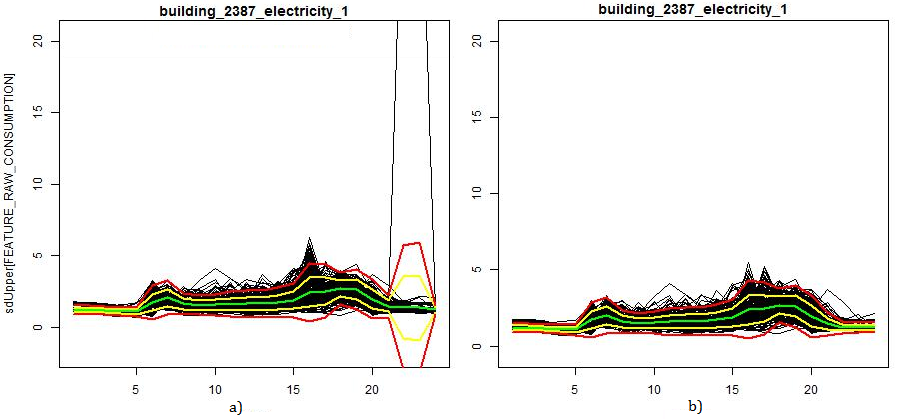
\includegraphics[scale=0.3]{outliereksempel.png}
\end{center}
\caption{Daytype profiles with and without outlier detection}
\end{figure}

The average number day types pr. building is 2.74 with a standard deviation of 0.95. This indicates that it is almost always possible to identify at least two distinct day types, namely working days and non working days. 

Often the best way to determine whatever a clustering was successful is to visually plot and inspect the results. Figure 6.3 shows two raw plots of two distinct day types for building 4297. The cluster plot to the right shows how they can be almost entirely separated using only two canonical variates, which explain 66.67\% of the point variability.
\begin{figure}
\begin{center}
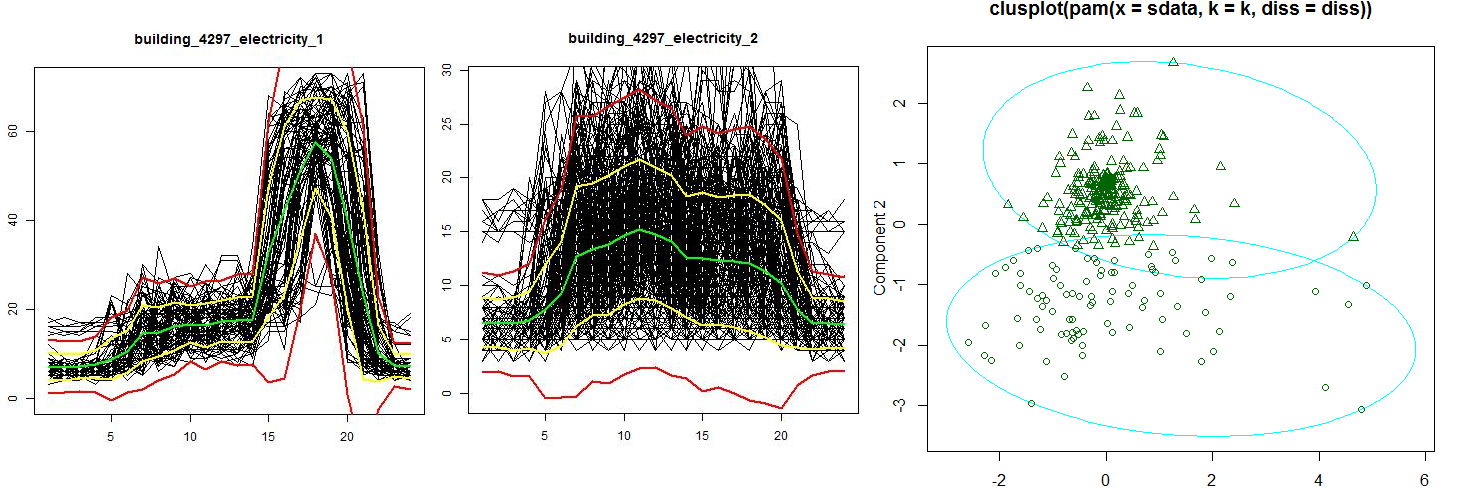
\includegraphics[scale=0.3]{comparingtwodaysclusterplot.png}
\end{center}
\caption{Two distinct day types and a cluster plot of the two day types}
\end{figure}

Appendix 11 -Daytype test setting contains 925 plots showing each of the day type profiles generated while running the test with setting number 5.

The clustering was additionally tried with the DBSCAN algorithm\footnote{See Related work and Methods} on various settings and features. However, this did not perform very well as it would often just create one single cluster. The clusterplot to the right on Figure 6.3 gives a hint as to why this is the case. Even though the two clusters seem very distinct from looking at the raw plots to the left, the cluster plot shows that they have overlap. If this overlap is too dense, then due to the way DBSCAN works they will come out as one single cluster.

\section*{Detection of faults}
Based on the day type profiles generated on the training data, the test data was checked for anomalies. The fault detection settings used was an alpha value of 0.05 and the features used for the fault detection were mean hourly consumption and nightly consumption. During the process buildings that did not have any daytype profiles due to missing data were discarded, and the same goes for days with missing values in the test data. The result was that 391 buildings were processed and in total 2435 days were checked for anomalies. In total 76 anomalies were detected of which 36 had to do with a higher than usual consumption. Figure 6.4 shows the detected anomalies spread across buildings.
\begin{figure}
\begin{center}
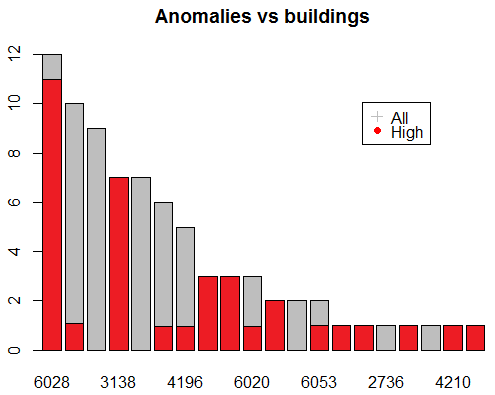
\includegraphics[scale=0.3]{anomaliesvsbuildings1.png}
\end{center}
\caption{Anormalies vs. Buildings}
\end{figure}

The 78 anomalies are spread across 20 buildings. Building 6028 has the largest number of anomalies, namely 12 from which 11 are due to a higher consumption. Investigating this issue further shows that the reason is a higher nightly consumption which is consistently above the means of its two daytype profiles. Figure 6.5 shows the two nightly consumption means from the daytype profiles (red lines). The blue lines are the maximum one can move up or down while still being within 2 standard deviations from any of the daytype profiles. The black line is building 6028's actual nightly consumption during the test month. The black line indicates that it has been higher than usual, because it is consistently above 2 standard deviations away from any of the daytype profiles.
\begin{figure}
\begin{center}
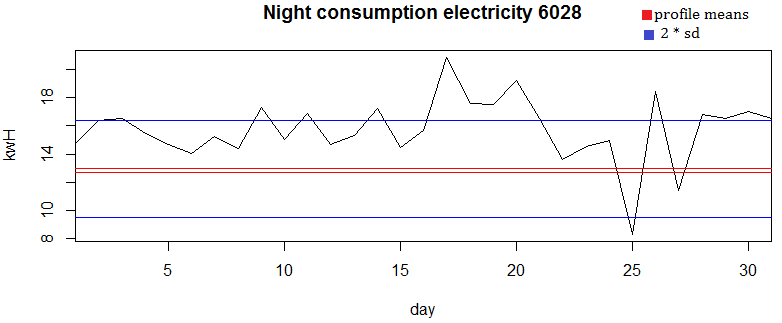
\includegraphics[scale=0.4]{nightconsumption6028.png}
\end{center}
\caption{The nightly electricity consumption of building 6028}
\end{figure}

Another way that the fault detection system was tested was to simulate a higher consumption and then see how many days would be detected as having this higher consumption. This test was run with a simulated increase in consumption from 0 - 100\%, and with $\alpha$ values 0.05 and 0.025. The results can be seen in figure 6.6.
\begin{figure}
\begin{center}
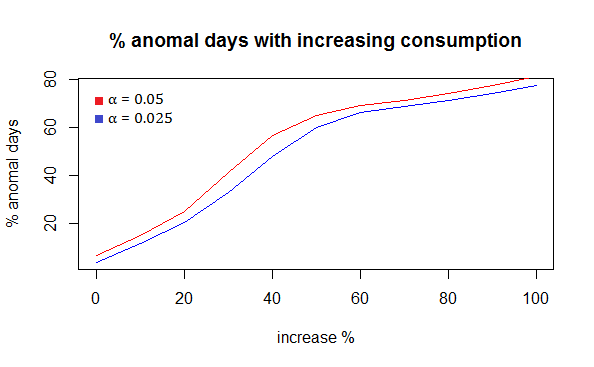
\includegraphics[scale=0.3]{anomalyvsincrease.png}
\end{center}
\caption{Simulated test of the fault detection}
\end{figure}
The figure shows that an for instance that a 20\% increase in overall consumption would be detected as an anomaly for roughly 20\% of all days. However the system could perform better on real data, because the increase would not be spread evenly across the entire day like the simulated increase.
\section*{Finding similar buildings}
This feature is somewhat difficult to evaluate since there is no clear metric for how similar two buildings in fact are. The approach will be to compare all buildings using the day type profiles generated in section $Daytype clustering$. These were generated using the training data, and thus the system finds similar buildings on basis of the training data. However for the evauluation of the systems performance the test data is used.

Using the training data the system compared all buildings and for each building the 30 most similar were noted. Figure 6.7 shows the raw electricity consumption of two different buildings during the test data month of March 2015. The black lines show the consumption of each building, and the red lines show the consumption of the 5 buildings that were rated as most similar to them. The plots show that the system did well in finding similar buildings. Appendix 12 -Similar Buildings contains a similar plot for each building that was used in the test.
\begin{figure}
\begin{center}
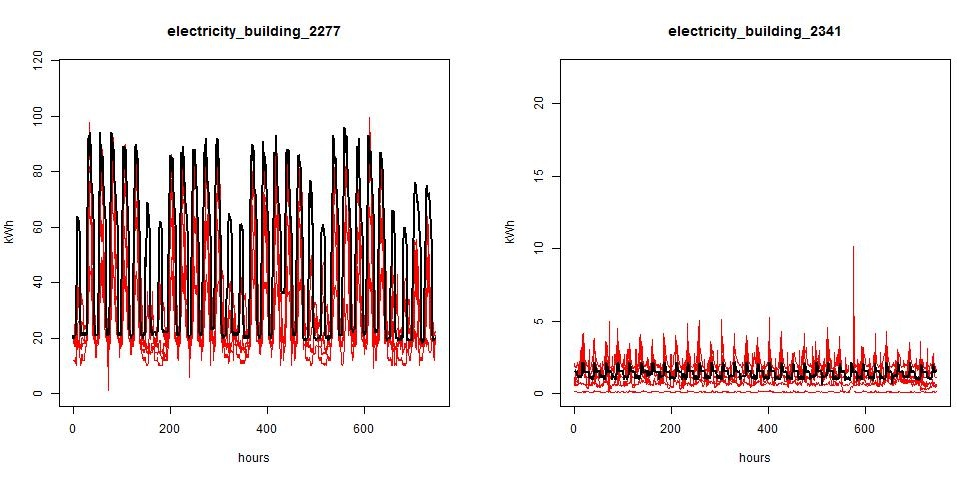
\includegraphics[scale=0.3]{electricity_building_2277.jpg}
\end{center}
\caption{Similarity of buildings consumption}
\end{figure}

Another way to test how well the system identifies similar buildings is to look at the properties of the buildings rated as similar rather than just the consumption figures. Unfortunately building properties like size, number of people, age of building etc. were too inconsistent in the dataset used. However the type of building (school, office, nursing home, etc.) was available for all buildings. Figure 6.8 shows for a selected number of building types how often buildings of those types appear as simmilar with other buildings. For instance the graph shows that buildings which are of type $integrated institution$ are on average similar with 7 other integrated institutions. While buildings which are not of this type are only similar with 3 integrated institutions on average. The shows that buildings of a given type, are more often rated as similar with other buildings of the same type.
\begin{figure}
\begin{center}
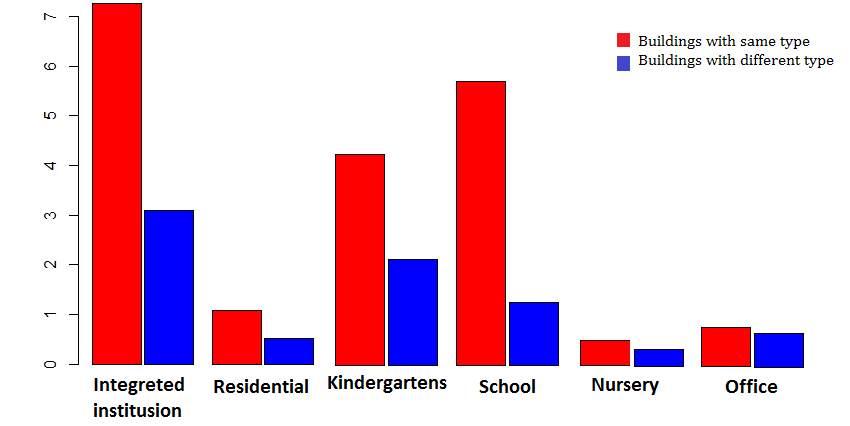
\includegraphics[scale=0.3]{plotsimmilarity2.png}
\end{center}
\caption{Similarity of buildings consumption}
\end{figure}
\section*{Integration of the system}
BEOVulf is fully automated in importing data from OM’s Energy Key system. Therefore it is possible from a data perspective to adopt the new system without any cost in effort for maintain multiple systems. However updates to informations in BEOVulf do not propagate to Energy Key. The two way integration on has not been made possible from the municipality, nor has it been a goal for this project. The system is currently only operating on 505 buildings, and have yet to import the buildings from the old SonWin\footnote{http://www.sonlinc.dk/sonwin.aspx} system. However, this tasks should be quite easy, since the developed system now have a implemented structure in which these data could be fitted into. 

Concerning the data quality in the developed system, some effective procedures have been developed which ensure that duplicated data entries can not occur. The database design along with the procedures ensure minimal usage of space and that data is consistent. All this ensures that the data quality is still the same when it is stored in the database, which again means that in order to improve data quality, the source needs to be improved, which has been out of scope for this project.
\section{Usability evaluation }
In order to test and verify the usability of the system, a representative from OM’s Energy and Maintenance department was interviewed.  He was a test pilot for the system, in a semi-supervised environment, where he was both using the system on his own, and also while being guided through some parts to ensure that he did not get stuck in the exploration of the system. Additionally, the guidance ensures that all features of the system were evaluated.
\section*{Learnability of system}
This section will evaluate how easy the system is to learn. This is of importance, because it addresses the effort needed from the user to become competent at carrying out tasks. If the system is easy to learn the adoption will be more smooth, the user, more efficient and it will lessens the change of the user making errors.

The test of the user interface showed that the visual design and concepts of the system were understood. The user was able to navigate around the page without help, showing that the current placement of the content is consistent with where the user expects it to be. This lessens the chance of confusion and undesirable experiences, like the frustration of getting lost or stuck.

The test showed that the content and information presented when viewing a single building is intuitive and recognizable to the user. It took the user a few seconds to look through the BBR informations and get an overview of the building information. The example shows that the quantity of information displayed is comprehensible. However, the test user did suggest that various panels could be collapsible, and that users with specific tasks should be able to have panels with irrelevant information to those tasks collapsed by default. Collapsible panels, have been a part of the original requirements and design plan, as mentioned in section Implementation of website. Therefore the system design can accommodate this feature with little change of the existing system. The ability for individual users to customize the interface was originally specified in requirement $F15-F17$, but was left out of scope for this project. However, the reaction expressed by the user can also be interpreted as a slightly confusion. This could indicate that the information presented is not intuitively enough to be interpreted on its own. This confusion might not be a problem for the power-user as it will expectedly decrease as the user learned or got used to the system, but if the system is to accommodate the general public, there will be a risk of the system being too advanced. In relation to this the following countermeasures might reduce the risk and increase the acceptance rate from the general public:
\begin{itemize}
\item Panels could be made visually more different from each other. This will make them more memorable and reduce the risk of users mixing up graphs
\item Panels could be made more self describing by addid guiding text on mouseover to different elements on the graph. 
\item A discrete help/information button could be added in the panel header, or alternatively as an expandable panel footer, with guiding/explaining text. 
\item Lastly, an alternative could be to introduce a tutorial for new users, where different elements could be explained. 
\end{itemize}
\paragraph{Comparing buildings:} 
On the building comparison page, the test user needed a little guidance at the beginning to understand what the right hand side bar was for. However the information needed to get him started was minimal, indicating that no additional helping functionality is needed and that the design works as intended. However, the test, showed that it is expected that clicking legend items will remove the item from the graph. This identified feature should be implemented in a further development, but is not found critical for the proof of concept prototype. The implementation of this feature in a further development will not affect the rest of the system, and will require little effort to implement.
\section*{Maintainability of the system and data}
This section will evaluate the maintainability of the system. It will elaborate on what effort is needed to maintain and sustain the system and the data quality wanted by the Energy and Maintenance department.   

Features for validating and changing existing data, have been included in the developed system, which means that the employees from the Energy and Maintenance department can verify and correct their data. These functionalities have also been tested both by the developers and the head of the department of Energy and Maintenance, and proven to be both easy and fast to use. As an example the head Energy and Maintenance answered the following when asked what was most important and if the system lacked any of this:
\begin{center}
"\emph{I’m just totally hooked on the feature with whether or not a building is validated}"\footnote{Appendix 03 -Meeting with Kim Allan 26-5-15: 7 minutes and 3 seconds in.}
\end{center}
This shows that is not always the big and advanced feature which creates the value for the user, but sometimes the features which are simple, small and easy to use. From this acceptance of the feature it have been concluded that the maintenance of the system data, will not burden the municipality with a lot of additional work.The head of the department of Energy and Maintenance stated that quite the contrary would be the consequence, because the timestamp on the panel would ensure that the personal did not do the same work twice as he expected they did quite often at the moment.
\section{Utility and efficiency of the product}
This section will evaluate the way the system supports the primary users in doing their tasks, and whether the system provides the right kind of functionality so that users can achieve their goals and sustain a high level of productivity. This section will start by looking at the page where the user can look at a specific building. From there it will move onto the page visualizing all alarms in the system, and lastly will it describe the comparison page. Lastly, this evaluation is based on the final test and interview.
\paragraph{Viewing a specific building}
After the representative from OM’s Energy and Maintenance department had tested the system, an interview was conducted which focussed on the department’s work and the possible applications of the system. In this discussion, it was found that the employees are mostly interested in whether or not the building is validated, rather than the informations themselves. Due to this, it was concluded that the panel took up too much space, and should be minimized when viewing a building after a validation. If this functionality is not implemented, in consequence this could lead to negative user experience, because employees will spend a great deal of time on scrolling past the panel.

Requirement $F2$, and its sub requirements, concretizes the visualization of a building. The feedback on these have showed it somewhat easier to see the behavioral patterns of a building in the developed system. Furthermore, when showing the test user a building, which the group members had discovered and found odd, it took the user less than a minute to see that something was in fact wrong. In addition it took him only few minutes before he had a list of probable causes. This shows the product does provide the tools necessary to identify problems and estimate their cause. Further, that the tools are more effective than those currently used. Unfortunately, there have been no time to test the software on a large scale, and therefore it can not be confirmed as a unique case or not. 

The test have found that the energy profiles is a powerful tool to obtain information of the behavioral patterns of a building. With this tool it is possible to learn a building's consumptions behavior in a matter of minutes instead of days/weeks. However, it seems that the presentation of these information can be improved, since the sliding and changing diagram can become annoying when a user is trying to read a chart/profile.

The test further showed that the seasonality functionality was an effective tool. The department of Energy and Maintenance makes these graphs, as a supporting tool for estimating the budget of a building. However, the software the department is currently using does not support them in generating these and therefore they currently have to create these graphs manually. When the Energy and Maintenance department was making the budgets for all 550 buildings, they tried creating these charts manually, but found it too time consuming and had to stop and find another procedure. Currently the procedure is to estimate with a professional guess. This makes a lot of space for making an human error. By introducing the autogenerated seasonality graph, the department of Energy and Maintenance would have the tool to create the budget based on facts, without acquiring additional effort. This would improve their current way of estimating the budgets for the buildings.

\paragraph{Alarms}
The test of the alarm feature revealed that error-code and error-messages along with visualization of observed consumption and normal consumption would be a very effective tool for the Department of Energy to diagnose the cause and analyse what counter action would be needed. Further the test concluded the department would save of time if they were using the developed alarming system. 

As for the page with all the alarms the test showed that it would support their workflow and support them in doing some of the more static tasks without too many mouse clicks. Based on this it have been concluded that the feature is accepted and that it will create value for the user.
\paragraph{Comparing buildings}
Regarding the page for comparing multiple consumption the test showed that the features are accepted by the user. Further it have been proven to be easier, faster and more flexible than the closest tool the department currently have at their disposal. The tool currently used is annoyingly slow, frustrating and do not provide the information in a very understandable way. 

The feature providing the possibility of plotting entire building types and compare these with a single building gives the department a new way of comparing and new understanding of the building. This feature was noted by the user, as a good way of giving a consumption context and perspective. 

As for the comparison features listed on the right side of the page, a change request was made. The system should support signed in user with functionality making it possible to change/define the feature. For example should it be possible to define which interval of the day should be used as the nightly consumption. This might be needed, because if the department of Energy are to trust what they see in the diagrams, then have to know what they are looking at. In addition, by creating a system where the user can change and interact more with the graph, the system will be more flexible and thereby accommodate more different tasks. Lastly, by creating a system where the user can see and change how a number is derived, it is easier for the user to understand and customize it to the user's specific needs.

Lastly, but unexpected the feedback from the test showed that the page/tool would help the department in localizing possible buildings for renovation. Further that the tool could provide a platform from which they could inspect/patrol many buildings faster than in their current system.